% =================================================================
% This is an assignment report template (in LaTeX) for the following course:
% PHYS 421 Parallel Computing
% Instructors: Sergiy Bubin, Bekdaulet Shukirgaliyev
% Version: 2025.08.10
% =================================================================

\documentclass[11pt,a4paper]{article}

% ---------- Encoding, fonts, language ----------
\usepackage[T1]{fontenc}
\usepackage[utf8]{inputenc}
\usepackage{lmodern}
\usepackage[english]{babel}

% ---------- Geometry & spacing ----------
\usepackage[a4paper,margin=1in]{geometry}
\usepackage{setspace}
\onehalfspacing
\usepackage{parskip} % space between paragraphs, no indent

% ---------- Math & symbols ----------
\usepackage{amsmath,amssymb,amsthm}
\usepackage{siunitx}
\sisetup{detect-all=true}

% ---------- Tables & graphics ----------
\usepackage{graphicx}
\usepackage{booktabs}
\usepackage{xcolor}
\usepackage{float}
\usepackage{subcaption}
\usepackage{mwe} % provides example-image-a
\usepackage{hologo}

% ---------- Hyperlinks & clever references ----------
%\usepackage[hidelinks]{hyperref}
\usepackage[colorlinks=true,urlcolor=blue,bookmarks=true,citecolor=magenta,breaklinks=true,pdftex]{hyperref}
\usepackage[nameinlink,capitalise]{cleveref}

% ---------- Code listings (default: listings) ----------
\usepackage{listings}
\lstdefinestyle{pcstyle}{
  basicstyle=\ttfamily\footnotesize,  %change \footnotesize to \small if the font in code snippets appears too small for reading
  numberstyle=\tiny, numbers=left, numbersep=8pt,
  showstringspaces=false, showtabs=false, showspaces=false,
  breaklines=true, frame=single, rulecolor=\color{black!20},
  keywordstyle=\color{blue!90!black},
  commentstyle=\color{green!65!black},
  stringstyle=\color{orange!80!black},
  tabsize=2,
  captionpos=b
}
\lstset{style=pcstyle}

% ---------- Optional: minted for code (requires shell-escape) ----------
% To use minted on Overleaf: Menu -> Latex -> Enable shell escape.
% Then uncomment the two lines below and comment out the listings section above.
% \usepackage[outputdir=_minted,cache=false]{minted}
% \setminted{fontsize=\small,breaklines,frame=single}

% ---------- PGFPlots for plots ----------
\usepackage{gincltex}
\usepackage{pgfplots}
\pgfplotsset{compat=1.18}
\usepackage{pgfplotstable}
\usepgflibrary{plotmarks}
\usetikzlibrary{calc}
\usetikzlibrary{positioning,arrows.meta}

% ---------- Bibliography ----------
\usepackage[
  backend=biber,
  style=numeric-comp, % compress ranges like [1–3]
  sorting=none,
  sortcites=true      % sort inside each \cite{...}
]{biblatex}
\addbibresource{references.bib}

% ---------- Utilities ----------
\usepackage{etoolbox} % for \IfFileExists

% ---------- Custom metadata commands ----------
% Replace X with the actual assignment number
\newcommand{\assignmentnumber}{X}
% Insert actual report title
\newcommand{\assignmenttitle}{Report Title}
% Insert your name
\newcommand{\studentname}{Askar Akhmetov}
% Replace XXXXXXXXX with your actual Student ID
\newcommand{\studentid}{XXXXXXXXX}
% Insert course code: PHYS 421, PHYS 521, or PHYS 721
\newcommand{\coursecode}{PHYS 421}  
% Insert course name: Parallel Computing or Parallel Programming for Scientific Computing
\newcommand{\coursename}{Parallel Computing} 

\newcommand{\honor}{I affirm that this work complies with Nazarbayev University academic integrity policies and the policies regarding the use of AI tools outlined in the course syllabus}

% ---------- Title ----------
\title{Assignment Report \#\assignmentnumber \\ \assignmenttitle}
\author{Student Name: \studentname \ (ID: \studentid) \\ Course: \coursecode \ \coursename
}
\date{Submitted: \today}

% =================================================================
\begin{document}
\maketitle

\begin{center}
{Software packages used:} \\
\begin{tabular}{|l|l|}
\hline
GCC 13.3.0               &  Main code \\
Open MPI 4.1.6           &  Main code, parallelization framework \\
LAPACK 3.12.0            &  Main code \\
Wolfram Mathematica 14.3 &  Analytical manipulations \\
\hline
\end{tabular}
\end{center}

\begin{center}
{AI tools used:} \\
\begin{tabular}{|l|l|}
\hline
ChatGPT-5           & Spellchecking, plotting figures, data analysis \\
Claude 4.1 Opus     & Coding assistance \\
Gemini 2.5 Pro      & Help with learning and understanding mathematical \\ 
                    & concepts  \\ 
DeepSeek-R1         & Data analysis \\
Github Copilot      & Coding assistance \\
\hline
\end{tabular}
\end{center}
\vspace{2em}

\begin{abstract}
\noindent
In the abstract, give a concise summary (4--8 sentences) of the problem studied, method used, hardware and software environment, key results, and main takeaways.
\end{abstract}
% =================================================================

\section{Introduction and Problem Statement}
The number of sections in the report, their titles, structure, etc., are up to the student.  
If necessary, you can divide the report into subsections (e.g., see Subsection~\ref{subsec:intr_content}) and subsubsections (e.g., see Subsubsection~\ref{subsubsec:highlighting}). If the report is short enoug, it may not warrant a complicated sectioning. Keep it simple, if possible.
There is are no requirements and/or limits on the length of the report. The suggested length is 5--10 pages, including title, abstract, graphics, tables, code snippets, appendices, etc. 

Throughout your report, you may need to cite journal articles, books, manuals, technical reports, web-pages, etc. This template uses \hologo{BibTeX}~for bibliography. Here we provide a couple of examples of references: \cite{rauber_course_textbook}, \cite{cuda_guide}, or \cite{golub_t_21_215_1979}. You can also combine several references in a single citation: \cite{rauber_course_textbook,cuda_guide,golub_t_21_215_1979}. Note that the reference information
is stored in a separate \texttt{references.bib} file, which you can modify, update, and use again with each new assignment.

\subsection{What Should Be in the Introduction?\label{subsec:intr_content}}

In the Introductory section clearly state the computational problem you deal in this assignment. Include mathematical formulation if relevant. Specify input sizes, data distributions, and expected outputs. Define what you expect to obtain and what questions you are looking to answer.

\subsubsection{Formatting and Highlighting\label{subsubsec:highlighting}}

When typesetting the report, feel free to use fonts (e.g. \textbf{Bold}, \textit{Italic}, \texttt{Typewriter}, \textsc{Small Caps}), colors (e.g. {\color{red}Red}, {\color{green} Green}, {\color{blue} Blue}, {\color{brown} Brown}, {\color{orange} Orange}), and relevant \LaTeX~environments to highlight different things. Most likely, you will need to use inline mathematical expressions, such as $c=\sqrt{a^2+b^2}$, or numbered equations, such as
\begin{equation}\label{eq:euler_formula}
e^{i x} = \cos x + i \sin x ,  
\end{equation}
or
\begin{equation}\label{eq:gaussian_integral}
\int\limits_{-\infty}^{+\infty} e^{- \alpha x^2} dx = \sqrt{\frac{\pi}{\alpha}},
\qquad
\mathrm{Re} \, \alpha > 0,
\end{equation}
which you can label and refer to in the text of the report. For example, the Euler formula given by Equation~(\ref{eq:euler_formula}) constitutes one of the most beautiful results in mathematics.  

\section{Hardware and Software Environment}
Include enough detail for the exact reproduction of your work. Find a place to mention all the software and libraries (including version numbers) that were used in the report. If you need to present data in a table form, below there is a small template (see Table~\ref{table:software_packages}) that you can adjust and expand as needed. 

\begin{table}[H]
  \centering
  \caption{A non-exhaustive list of software packages available in Ubuntu 24.04 that will be used in PHYS 421 Parallel Computing.}
  \label{table:software_packages}
  \begin{tabular}{lll}
    \toprule
    Software Package  & Version & Installation command \\
    \midrule
    GCC   &  13.3.0  &  \texttt{sudo apt install build-essential} \\
    Open MPI                        &  4.1.6   &  \texttt{sudo apt install libopenmpi-dev openmpi-bin} \\
    LAPACK &  3.12.0  &  \texttt{sudo apt install liblapack-dev libblas-dev}\\
    \bottomrule
  \end{tabular}
\end{table}

\section{Methods and Implementation}
Describe your approach clearly. For example, if you write a parallel code explain the domain decomposition, work partitioning, data layout, communication patterns, and key synchronization points. If you wish, you can provide a pseudocode or short code excerpts where helpful. An example code excerpt containing a simple ``Hello, world!'' program is given in Listing~\ref{lst:hello_c}. 
Please be mindful of inserting very long code fragments though. Remember that your entire source code (in one or multiple files) will be part of the assignment submission anyway.

\begin{lstlisting}[language=C, caption={Hello World in C}, label={lst:hello_c}]
#include <stdio.h>

int main(void) {
    printf("Hello, world!\n");
    return 0;
}
\end{lstlisting}


\subsection{Build and Run Instructions}
Remember that the code you submit must be compilable. If the code is not compilable, your assignment
score will be very low, if not zero. In order to avoid any confusion, be sure
to provide exact commands to compile your code and reproduce your results. For example, you could include a Bash snippet such as the one given in Listing~\ref{lst:commands} below:
\begin{lstlisting}[language=bash,caption={Build and run commands.},label={lst:commands}]
# Build (example for MPI + OpenMP)
module load gcc/13.2 openmpi/4.1.6
mpicxx -O3 -march=native -fopenmp -DNDEBUG -o matmul src/matmul.cpp

# Run (30 MPI ranks, 4 OpenMP threads each)
export OMP_NUM_THREADS=4
srun -N 3 -n 30 --cpus-per-task=4 --hint=nomultithread ./matmul --n 8192
\end{lstlisting}

\subsection{Code and Data Organization}
Briefly explain the structure of your source code and data, i.e., what each file contains. Be mindful of submitting excessively large data files. If anything that you submit exceeds, say, 10 MB in size, then you should seriously think if it is absolutely necessary. 


\section{Results}
Present numerical results, validation checks, and representative outputs. Use tables for small data and plots for scaling trends.

\subsection{Correctness and Validation}
Explain how you verified correctness (for example, norms, checksums, unit tests, convergence tests). Report any discrepancies and their causes.

\subsection{Performance Metrics}
Report wall-clock time, throughput, speedup, parallel efficiency, memory bandwidth, and GPU occupancy when relevant. Define precisely how you computed each metric.

\begin{table}[H]
  \centering
  \caption{Example timing summary (strong scaling).}
  \begin{tabular}{rrrrr}
    \toprule
    Ranks & Threads per rank & Time (s) & Speedup & Efficiency (\%) \\
    \midrule
    1 & 2 & 120.1 & 1.00 & 100 \\
    2 & 2 & 61.0 & 1.97 & 98 \\
    4 & 2 & 31.5 & 3.81 & 95 \\
    6 & 2 & 21.7 & 5.53 & 92 \\    
    8 & 2 & 16.8 & 7.15 & 89 \\
    \bottomrule
  \end{tabular}
  \label{table:timings}
\end{table}

\subsection{Graphics}
Include graphics that illustrate your results. If the graphics are plots of data or functions, make sure to label axes and units. 

\subsubsection{JPG or PNG images}
You can include images in JPG or PNG format, such as this portrait of P. Dirac in Figure~\ref{fig:dirac}. Ensure that all raster images have a resolution of at least 200  (dots per inch) and preferably 300 DPI. For example, if your image is half-page wide, then its horizontal resolution should be around 300*8.27/2=1240 pixels or so in order to meet the 300 DPI requirement.

\begin{figure}[H]
    \centering
    \includegraphics[width=2.0in]{fig_portrait.jpg}
    \caption{Paul Adrien Maurice Dirac was an English theoretical physicist and mathematician who is considered to be one of the founders of quantum mechanics (image credit: Wikipedia).}
    \label{fig:dirac}
\end{figure}

\subsubsection{Tikzpicture}
If you have a data plot (e.g., execution time vs number of CPU cores) you can generate it in a raster format such as JPG or PNG, just like the portrait in Figure~\ref{fig:dirac}. However, the figure will be of higher quality if you generate it in a vector format. One of the possible ways to do it is to
use the \texttt{tikzpicture} environment. Figure~\ref{fig:data_points} shows an example of a plot based on the data in Table~\ref{table:timings}.  

\begin{figure}[H]
    \centering
    \includegraphics[width=0.7\linewidth]{fig_plot_data_points.tex} 
    \caption{A sample plot that shows a few discrete data points.}
    \label{fig:data_points}
\end{figure}

It is also easy to plot mathematical functions within \texttt{tikzpicture} environment. 
Figure~\ref{fig:plot_of_function} demonstrates this.

\begin{figure}[H]
  \centering
  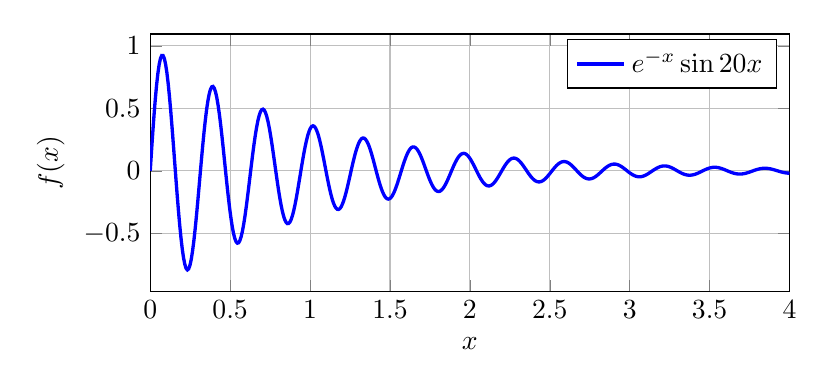
\begin{tikzpicture}
    \begin{axis}[
      width=0.8\linewidth,
      height=0.4\linewidth,
      xlabel={$x$}, ylabel={$f(x)$},
      domain=0:4, samples=500,
      xmin=0, xmax=4,
      enlarge x limits=false,   % no extra padding beyond [0,5]
      restrict x to domain=0:4, % clip any stray bits to [0,5]
      grid=both
    ]
      \addplot+[mark=none, color=blue, line width=1.2pt]
        {sin(20*deg(x)) * exp(-x)};
      \addlegendentry{$e^{-x} \sin 20x$}
    \end{axis}
  \end{tikzpicture}
  \caption{Plot of $f(x) = e^{-x} \sin 20x$ on the interval $[0,4]$ using PGFPlots/TikZ.}
  \label{fig:plot_of_function}
\end{figure}

A common type of graphics that may be relevant when discussing algorithms is a block scheme. 
An example of a block scheme generated within the \texttt{tikzpicture} environment is given in Figure~\ref{fig:block_scheme_branch}.

\begin{figure}[H]
\centering
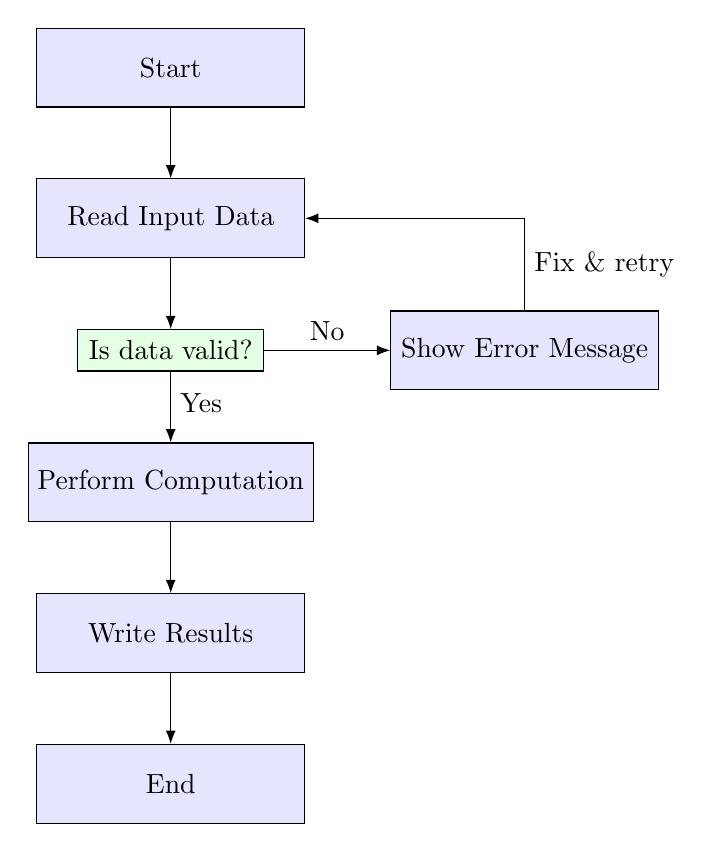
\begin{tikzpicture}[
  node distance=0.9cm and 1.6cm,
  >=Latex,                % set default arrow tip
  block/.style={rectangle, draw, fill=blue!10, minimum height=10mm, minimum width=34mm, align=center},
  decision/.style={rectangle, draw, fill=green!10, inner sep=4pt, align=center}
]
% Nodes
\node[block]                         (start)  {Start};
\node[block,    below=of start]      (input)  {Read Input Data};
\node[decision, below=of input]      (check)  {Is data valid?};
\node[block,    right=of check]      (error)  {Show Error Message};
\node[block,    below=of check]      (process){Perform Computation};
\node[block,    below=of process]    (output) {Write Results};
\node[block,    below=of output]     (stop)   {End};

% Edges
\draw[->] (start)  -- (input);
\draw[->] (input)  -- (check);
\draw[->] (check)  -- node[right,pos=0.45]{Yes} (process);
\draw[->] (check.east) -- node[above]{No} (error.west);
\draw[->] (error) |- node[pos=0.25,right]{Fix \& retry} (input.east);
\draw[->] (process) -- (output);
\draw[->] (output)  -- (stop);
\end{tikzpicture}
\caption{A simple block scheme with a decision branch and a loop on invalid input.}
\label{fig:block_scheme_branch}
\end{figure}

You can use \texttt{tikzpicture} environments to create figures containing all kind of objects and shapes. 
It is limited by your imagination and the time you want to spend on it (the time can be greatly reduced if you use AI tools to help yourself). 
An example is given in Figure~\ref{fig:coordinates_bh}, which shows how internal coordinates are defined in the boron hydride molecule.

\begin{figure}[H]
    \centering
    \includegraphics[width=0.5\linewidth]{fig_coordinates.tex} 
    \caption{Internal coordinates of the electrons and proton in the BH molecule.}
    \label{fig:coordinates_bh}
\end{figure}

\section{Discussion}
Interpret the results, indicate bottlenecks (e.g., Amdahl's law, load imbalance, communication versus computation overlap, memory bandwidth, etc), and how code or runtime settings affected performance. Include evidence when possible.

\section{Reproducibility}
In your submission, provide everything needed for instructors to  your results: input generation steps, random seeds, environment modules, SLURM script files (see example in Listing~\ref{lst:slurm_script}), Makefiles, and exact command lines. If datasets are large, provide a small test case and a script to regenerate full-size inputs.

\subsection{SLURM Script (example)}
\begin{lstlisting}[language=bash,caption={Example SLURM submission script.},label={lst:slurm_script}]
#!/bin/bash
#SBATCH --job-name=My_A0_job 
#SBATCH --time=0-0:30:00 
#SBATCH --mem=1G 
#SBATCH --nodes=1 
#SBATCH --ntasks=1 
#SBATCH --cpus-per-task=128 
#SBATCH --partition=CPU 
#SBATCH --output=stdout%j.out
#SBATCH --error=stderr%j.out
#SBATCH --mail-type=END,FAIL
#SBATCH --mail-user=your.name@nu.edu.kz

# Load module GCC 13.2
module load GCC/13.2.0

# Set the number of threads for OpenMP to match the cpus-per-task directive
export OMP_NUM_THREADS=$SLURM_CPUS_PER_TASK

# Run the program
./my_smp_program
\end{lstlisting}

\subsection{Build Configuration}
List compiler flags and variants tested. Example CMake invocation:
\begin{lstlisting}[language=bash,caption={CMake build variants.}]
cmake -S . -B build/Release -DCMAKE_BUILD_TYPE=Release -DUSE_OPENMP=ON
cmake --build build/Release -j
\end{lstlisting}

\section{Conclusion}
Summarize the key performance achievements and one or two specific next steps that would most likely improve performance further.

\section*{Acknowledgments}
Credit collaborators, libraries, and online resources you used.

\section*{Honor Statement}
\honor

\printbibliography

\section*{Submission Checklist}
\begin{itemize}
  \item PDF file of the report named \texttt{report\_aX\_lastname.pdf}, where \texttt{X} stands for the assignment number, is absolutely required. 
  Optionally, you may also include the \LaTeX~source code and figures. If you do so, make sure it compiles without errors.
  \item Source code of your main program. Again, make sure it is compilable.
  \item A short \texttt{README.md} (file in Markdown format, preferred) or \texttt{README.txt} (plain ASCII text file) that includes build and run instructions.
  \item Any data files required for execution (if applicable).
  \item SLURM scripts (if applicable) or exact command lines.
  \item Random seeds and environment details recorded for reproducibility (if applicable).
\end{itemize}

% ---------- Appendix ----------
\appendix
\section{Additional Figures and Tables}
Add any supplementary plots, tables, listings, etc. as appendices, if necessary. The appendices typically include things that are not essential for reading and understanding the main document, but rather contain auxiliary information.

\section{Another Appendix}
Add any supplementary plots, tables, listings, etc. as appendices, if necessary. The appendices typically include things that are not essential for reading and understanding the main document, but rather contain auxiliary information.

\end{document}